
\section{Three Point Perspective Drawing Library}

\noindent\emph{by Max Snippe}

\begin{tikzlibrary}{perspective}
  This library provides tools for perspective drawing with one, two, or three
  vanishing points.
\end{tikzlibrary}
%
\begin{codeexample}[setup code,hidden]
    \usetikzlibrary{perspective}
\end{codeexample}


\subsection{Coordinate Systems}

\begin{coordinatesystem}{three point perspective}
  The |three point perspective| coordinate system is very similar to the |xyz|
  coordinate system, save that it will display the provided coordinates with a
  perspective projection.
  %
  \begin{key}{/tikz/cs/x=\meta{number} (initially 0)}
    The $x$ component of the coordinate. Should be given \emph{without} unit.
  \end{key}
  %
  \begin{key}{/tikz/cs/y=\meta{number} (initially 0)}
    Same as |x|.
  \end{key}
  %
  \begin{key}{/tikz/cs/z=\meta{number} (initially 0)}
    Same as |x|.
  \end{key}
\end{coordinatesystem}

\begin{coordinatesystem}{tpp}
  The |tpp| coordinate system is an alias for the |three point perspective|
  coordinate system.
\end{coordinatesystem}


\subsection{Setting the view}

\begin{key}{/tikz/3d view=\marg{azimuth}\marg{elevation}
    (default \{-30\}\{15\})}
  With the |3d view| option, the projection of the 3D coordinates on the 2D page
  is defined. It is determined by rotating the coordinate system by
  $-\meta{azimuth}$ around the $z$-axis, and by \meta{elevation} around the
  (new) $x$-axis, as shown below.

  \begin{tikzpicture}[
    viewpoint/.pic={
      \draw (22.5:0.45) -- (0,0) -- (-22.5:0.45);
      \draw (0,0) ++ (22.5:0.35) arc (22.5:-22.5:0.35);
      \draw (0.225,0) circle (0.02 and 0.09);
    }]
    \begin{scope}[3d view={-20}{20}]
      \draw[->] (-3,0,0) -- (3,0,0) node[pos=1.05]{x};
      \draw[->] (0,-3,0) -- (0,3,0) node[pos=1.05]{y};
      \draw[->] (0,0,-1) -- (0,0,3) node[pos=1.05]{z};

      \pgfmathsetmacro\az{50}
      \begin{scope}[canvas is xy plane at z=0]
        \draw[->] (0,0) ++(0,-2) arc (-90:-90+\az:2) coordinate[pos=0.5](az);
        \draw (az) -- ++(-90+\az/2:1) node[below]{\meta{azimuth}};
        \draw[dashed] (0,0) -- ++(-90+\az:3);
      \end{scope}
      \begin{scope}[rotate around z=\az]
        \pgfmathsetmacro\el{50}
        \begin{scope}[canvas is yz plane at x=0]
          \draw[->] (0,0) ++(-2.5,0) arc (180:180-\el:2.5)
            coordinate[pos=0.5](el);
          \draw (el) -- ++(180-\el/2:1) node[above]{\meta{elevation}};
          \draw[dashed] (0,0) --
            pic[solid,sloped,transform shape,pos=1.2]{viewpoint} ++(180-\el:3);
        \end{scope}
      \end{scope}
    \end{scope}
  \end{tikzpicture}

  For example, when both \meta{azimuth} and \meta{elevation} are 0$^\circ$,
  $+z$ will be pointing upward, and $+x$ will be pointing right. The default is
  as shown below.
  %
\begin{codeexample}[]
\begin{tikzpicture}[3d view]
  \draw[->] (-1,0,0) -- (1,0,0) node[pos=1.1]{x};
  \draw[->] (0,-1,0) -- (0,1,0) node[pos=1.1]{y};
  \draw[->] (0,0,-1) -- (0,0,1) node[pos=1.1]{z};
\end{tikzpicture}
\end{codeexample}
\end{key}

\begin{stylekey}{/tikz/isometric view}
  A special kind of |3d view| is isometric, which can be set with the
  |isometric view| style. It simply sets |3d view={-45}{35.26}|. The value for
  \meta{elevation} is determined with $\arctan(1/\sqrt{2})$. In isometric
  projection the angle between any pair of axes is 120$^\circ$, as shown below.
\begin{codeexample}[]
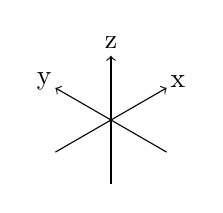
\begin{tikzpicture}[isometric view]
  \draw[->] (-1,0,0) -- (1,0,0) node[pos=1.1]{x};
  \draw[->] (0,-1,0) -- (0,1,0) node[pos=1.1]{y};
  \draw[->] (0,0,-1) -- (0,0,1) node[pos=1.1]{z};
\end{tikzpicture}
\end{codeexample}
\end{stylekey}


\subsection{Defining the perspective}

\begin{codeexample}[setup code,hidden]
\newcommand\simplecuboid[3]{%
  \fill[gray!80!white] (tpp cs:x=0,y=0,z=#3)
    -- (tpp cs:x=0,y=#2,z=#3)
    -- (tpp cs:x=#1,y=#2,z=#3)
    -- (tpp cs:x=#1,y=0,z=#3) -- cycle;
  \fill[gray]  (tpp cs:x=0,y=0,z=0)
    -- (tpp cs:x=0,y=0,z=#3)
    -- (tpp cs:x=0,y=#2,z=#3)
    -- (tpp cs:x=0,y=#2,z=0) -- cycle;
  \fill[gray!50!white] (tpp cs:x=0,y=0,z=0)
    -- (tpp cs:x=0,y=0,z=#3)
    -- (tpp cs:x=#1,y=0,z=#3)
    -- (tpp cs:x=#1,y=0,z=0) -- cycle;}

\newcommand{\simpleaxes}[3]{%
  \draw[->] (-0.5,0,0) -- (#1,0,0) node[pos=1.1]{x};
  \draw[->] (0,-0.5,0) -- (0,#2,0) node[pos=1.1]{y};
  \draw[->] (0,0,-0.5) -- (0,0,#3) node[pos=1.1]{z};}
\end{codeexample}

In this section, the following example cuboid will be used with various scaling.
As a reference, the axes will be shown too, without perspective projection.
%
\begingroup
\let\simplecuboid\relax
\let\simpleaxes\relax
\begin{codeexample}[]
\newcommand\simplecuboid[3]{%
  \fill[gray!80!white] (tpp cs:x=0,y=0,z=#3)
    -- (tpp cs:x=0,y=#2,z=#3)
    -- (tpp cs:x=#1,y=#2,z=#3)
    -- (tpp cs:x=#1,y=0,z=#3) -- cycle;
  \fill[gray]  (tpp cs:x=0,y=0,z=0)
    -- (tpp cs:x=0,y=0,z=#3)
    -- (tpp cs:x=0,y=#2,z=#3)
    -- (tpp cs:x=0,y=#2,z=0) -- cycle;
  \fill[gray!50!white] (tpp cs:x=0,y=0,z=0)
    -- (tpp cs:x=0,y=0,z=#3)
    -- (tpp cs:x=#1,y=0,z=#3)
    -- (tpp cs:x=#1,y=0,z=0) -- cycle;}
\newcommand{\simpleaxes}[3]{%
  \draw[->] (-0.5,0,0) -- (#1,0,0) node[pos=1.1]{x};
  \draw[->] (0,-0.5,0) -- (0,#2,0) node[pos=1.1]{y};
  \draw[->] (0,0,-0.5) -- (0,0,#3) node[pos=1.1]{z};}

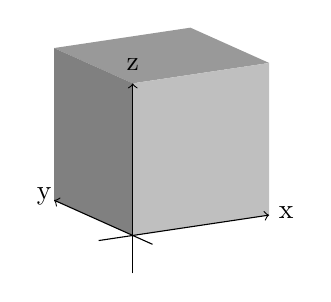
\begin{tikzpicture}[3d view]
  \simplecuboid{2}{2}{2}
  \simpleaxes{2}{2}{2}
\end{tikzpicture}
\end{codeexample}
\endgroup

\begin{key}{/tikz/perspective=\meta{vanishing points}
    (default p=\{(10,0,0)\},q=\{(0,10,0)\},r=\{(0,0,20)\})}
  The `strength' of the perspective can be determined by setting the location of
  the vanishing points. The default values have a stronger perspective towards
  $x$ and $y$ than towards $z$, as shown below.
  %
\begin{codeexample}[]
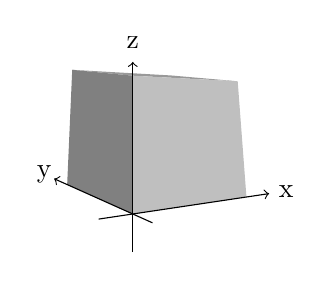
\begin{tikzpicture}[3d view,perspective]
  \simplecuboid{2}{2}{2}
  \simpleaxes{2}{2}{2}
\end{tikzpicture}
\end{codeexample}
%
  From this example it also shows that the maximum dimensions of the cuboid are
  no longer 2 by 2 by 2. This is inherent to the perspective projection.
  %
  \begin{key}{/tikz/perspective/p=\marg{x,y,z} (initially (0,0,0))}
    The location of the vanishing point that determines the `strength' of the
    perspective in $x$-direction can be set with the |p| key.
    %
\begin{codeexample}[]
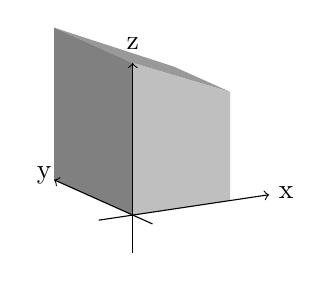
\begin{tikzpicture}[
  3d view,
  perspective={
    p = {(5,0,0)}}]
  \simplecuboid{2}{2}{2}
  \simpleaxes{2}{2}{2}
\end{tikzpicture}
\end{codeexample}
    %
    Note also that when only |p| is provided, the perspective in $y$ and $z$
    direction is turned off.

    To turn of the perspective in $x$-direction, one must set the $x$ component
    of |p| to \texttt{0} (e.g. |p={(0,a,b)}|, where \texttt{a} and \texttt{b}
    can be any number and will be ignored). Or one can provide |q| and |r| and
    omit |p|.

    By changing the $y$ and $z$ components of |p|, one can achieve various
    effects.
    %
\begin{codeexample}[]
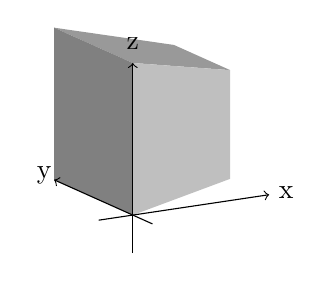
\begin{tikzpicture}[
  3d view,
  perspective={
    p = {(5,0,1)}}]
  \simplecuboid{2}{2}{2}
  \simpleaxes{2}{2}{2}
\end{tikzpicture}
\end{codeexample}
    %
\begin{codeexample}[]
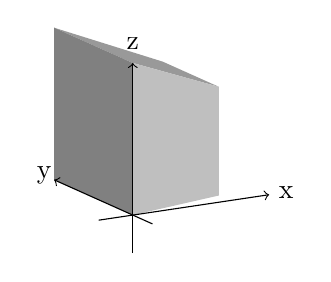
\begin{tikzpicture}[
  3d view,
  perspective={
    p = {(5,1,0)}}]
  \simplecuboid{2}{2}{2}
  \simpleaxes{2}{2}{2}
\end{tikzpicture}
\end{codeexample}
    %
\begin{codeexample}[]
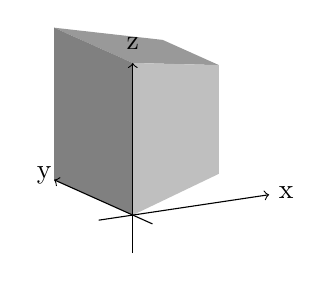
\begin{tikzpicture}[
  3d view,
  perspective={
    p = {(5,1,1)}}]
  \simplecuboid{2}{2}{2}
  \simpleaxes{2}{2}{2}
\end{tikzpicture}
\end{codeexample}
    %
  \end{key}
  %
  \begin{key}{/tikz/perspective/q=\marg{x,y,z} (initially (0,0,0))}
    Similar to |p|, but can be turned off by setting its $y$ component to
    \texttt{0}.
    %
\begin{codeexample}[]
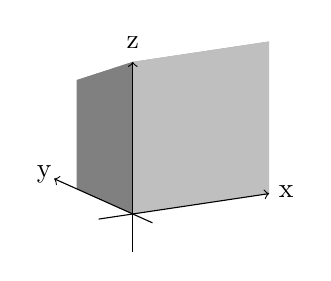
\begin{tikzpicture}[
  3d view,
  perspective={
    q = {(0,5,0)}}]
  \simplecuboid{2}{2}{2}
  \simpleaxes{2}{2}{2}
\end{tikzpicture}
\end{codeexample}
    %
  \end{key}
  %
  \begin{key}{/tikz/perspective/r=\marg{x,y,z} (initially (0,0,0))}
    Similar to |p|, but can be turned off by setting its $z$ component to
    \texttt{0}.
    %
\begin{codeexample}[]
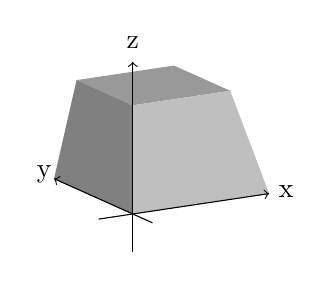
\begin{tikzpicture}[
  3d view,
  perspective={
    r = {(0,0,5)}}]
  \simplecuboid{2}{2}{2}
  \simpleaxes{2}{2}{2}
\end{tikzpicture}
\end{codeexample}
    %
  \end{key}
\end{key}


\subsection{Shortcomings}

Currently a number of things are not working, mostly due to the fact that PGF
uses a 2D coordinate system underwater, and perspective projection is a
non-linear affine transformation which needs to be aware of all three
coordinates. These three coordinates are currently lost when processing a 3D
coordinate.
The issues include, but possibly are not limited to:
%
\begin{itemize}
    \item Keys like |shift|, |xshift|, |yshift| are not working
    \item Keys like |rotate around x|, |rotate around y|, and |rotate around z|
      are not working
    \item Units are not working
    \item Most keys from the |3d| library are unsupported, e.g. all the
      |canvas is .. plane| keys.
\end{itemize}


\subsection{Examples}

An |r| that lies `below' your drawing can mimic a macro effect.
%
\nopagebreak
\begin{codeexample}[]
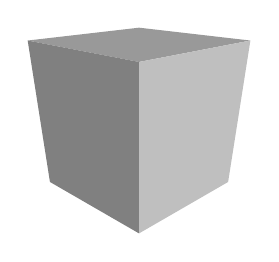
\begin{tikzpicture}[
  isometric view,
  perspective={
    p = {(8,0,0)},
    q = {(0,8,0)},
    r = {(0,0,-8)}}]

  \simplecuboid{2}{2}{2}]

\end{tikzpicture}
\end{codeexample}

A peculiar phenomenon inherent to perspective drawing, is that however great
your coordinate will become in the direction of the vanishing point, it will
never reach it.
%
\nopagebreak
\begin{codeexample}[]
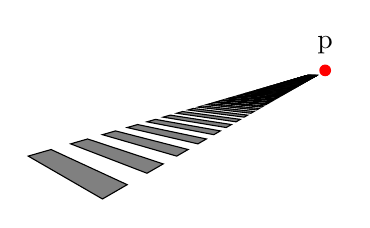
\begin{tikzpicture}[
  isometric view,
  perspective={
    p = {(4,0,0)},
    q = {(0,4,0)}}]

    \node[fill=red,circle,inner sep=1.5pt,label=above:p] at (4,0,0){};

    \foreach \i in {0,...,100}{
      \filldraw[fill = gray] (tpp cs:x=\i,y=0,z=0)
        -- (tpp cs:x=\i+0.5,y=0,z=0)
        -- (tpp cs:x=\i+0.5,y=2,z=0)
        -- (tpp cs:x=\i,y=2,z=0)
        -- cycle;}
\end{tikzpicture}
\end{codeexample}

Even for simple examples, the added perspective might add another `dimension' to
your drawing. In this case, two vanishing points give a more intuitive result
then three would.
%
\nopagebreak
\begin{codeexample}[]
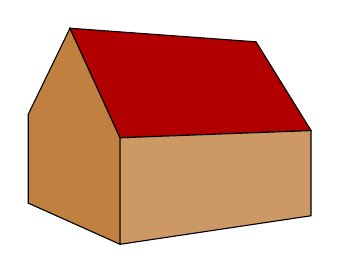
\begin{tikzpicture}[
  scale=0.7,
  3d view,
  perspective={
    p = {(20,0,0)},
    q = {(0,20,0)}}]

  \filldraw[fill=brown] (tpp cs:x=0,y=0,z=0)
    -- (tpp cs:x=0,y=4,z=0)
    -- (tpp cs:x=0,y=4,z=2)
    -- (tpp cs:x=0,y=2,z=4)
    -- (tpp cs:x=0,y=0,z=2) -- cycle;
  \filldraw[fill=red!70!black] (tpp cs:x=0,y=0,z=2)
    -- (tpp cs:x=5,y=0,z=2)
    -- (tpp cs:x=5,y=2,z=4)
    -- (tpp cs:x=0,y=2,z=4) -- cycle;
  \filldraw[fill=brown!80!white] (tpp cs:x=0,y=0,z=0)
    -- (tpp cs:x=0,y=0,z=2)
    -- (tpp cs:x=5,y=0,z=2)
    -- (tpp cs:x=5,y=0,z=0) -- cycle;
\end{tikzpicture}
\end{codeexample}

With the vanishing points nearby, the distortion of parallel lines becomes very
strong. This might lead to \texttt{Dimension too large} errors.
%
\nopagebreak
\begin{codeexample}[]
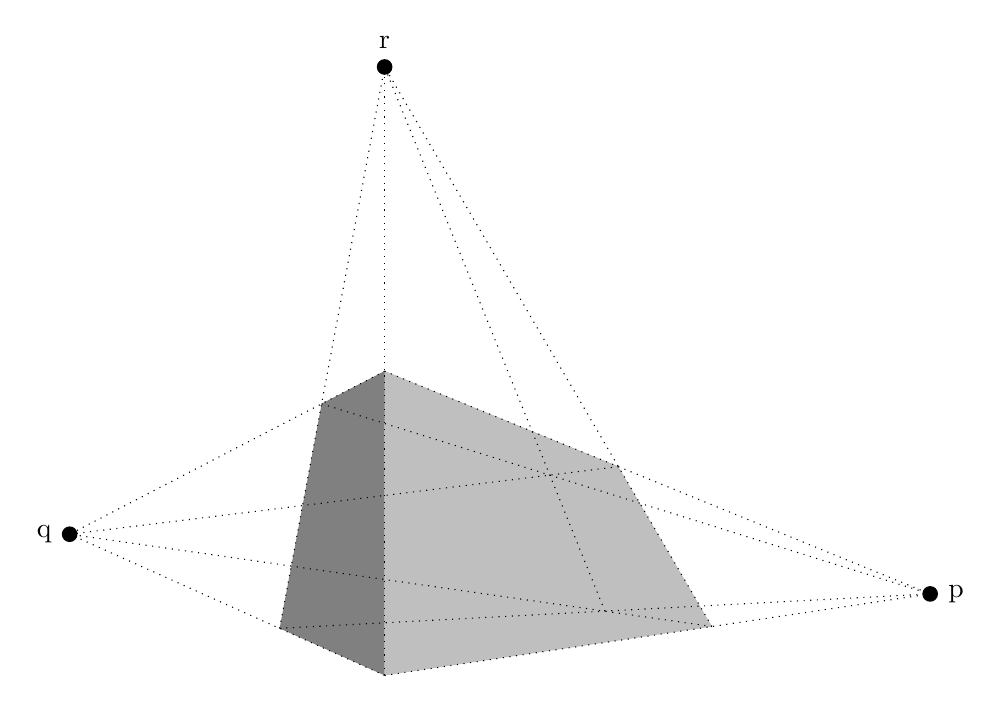
\begin{tikzpicture}[
  3d view,
  perspective={
    p = {(2,0,0)},
    q = {(0,2,0)},
    r = {(0,0,2)}},
  scale=4,
  vanishing point/.style={fill,circle,inner sep=2pt}]

  \simplecuboid{3}{1}{2}

  \node[vanishing point,label = right:p] (p) at (2,0,0){};
  \node[vanishing point,label = left:q] (q) at (0,2,0){};
  \node[vanishing point,label = above:r] (r) at (0,0,2){};

  \begin{scope}[dotted]
    \foreach \y in {0,1}{
      \foreach \z in {0,2}{
        \draw (tpp cs:x=0,y=\y,z=\z) -- (p.center);}}
    \foreach \x in {0,3}{
      \foreach \z in {0,2}{
        \draw (tpp cs:x=\x,y=0,z=\z) -- (q.center);}}
    \foreach \x in {0,3}{
      \foreach \y in {0,1}{
        \draw (tpp cs:x=\x,y=\y,z=0) -- (r.center);}}
  \end{scope}
\end{tikzpicture}
\end{codeexample}

% A more complex example.
\iffalse
Of course these examples can become as complex as desired, but as with any 3D
drawing using \tikzname, the order of drawing commands is important and can
become increasingly more complex.
%
\nopagebreak
\begin{codeexample}[]
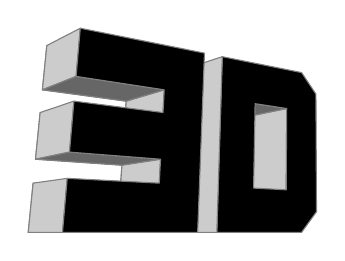
\begin{tikzpicture}[
  cycle of vertices/.style 2 args={
    insert path={
      foreach \i [count=\j,evaluate=\j as \k using
        {ifthenelse(\j==1,"","-- "}] in {#2}{\k (vert-#1-\i)} -- cycle}},
  scale=0.7,
  line join=round,
  bottom/.style={draw=white!50!black,fill=white!40!black},
  front/.style={draw=white!50!black,fill=black},
  side/.style={draw=white!50!black,fill=white!80!black},
]
  \begin{scope}[
    3d view={-20}{0},
    perspective={
      p = {(20,0,0)},
      q = {(0,20,0)},
      r = {(5,1,50)},
    }]
    \path foreach \x/\y/\z [count=\i] in {
      3.5/2.0/0.0,3.5/2.0/4.0,6.0/2.0/4.0,6.5/2.0/3.5,6.5/2.0/0.5,6.0/2.0/0.0,
      4.5/2.0/1.0,4.5/2.0/3.0,5.5/2.0/3.0,5.5/2.0/1.0,3.5/0.0/0.0,3.5/0.0/4.0,
      6.0/0.0/4.0,6.5/0.0/3.5,6.5/0.0/0.5,6.0/0.0/0.0,4.5/0.0/1.0,4.5/0.0/3.0,
      5.5/0.0/3.0,5.5/0.0/1.0%
    }{(tpp cs:x=\x,y=\y,z=\z) coordinate[name=vert-D-\i]};
    \filldraw[front,cycle of vertices={D}{1,...,6},
      cycle of vertices={D}{7,10,9,8}];
    \filldraw[side,cycle of vertices={D}{10,9,19,20}];
    \filldraw[bottom,cycle of vertices={D}{8,9,19,18}];
    \filldraw[front,cycle of vertices={D}{11,...,16},
      cycle of vertices={D}{17,20,19,18}];
    \filldraw[side,cycle of vertices={D}{1,2,12,11}];
    % '3'
    \path foreach \x/\y/\z [count=\i] in {
      0.0/2.0/0.0,0.0/2.0/1.0,2.0/2.0/1.0,2.0/2.0/1.5,0.0/2.0/1.5,0.0/2.0/2.5,
      2.0/2.0/2.5,2.0/2.0/3.0,0.0/2.0/3.0,0.0/2.0/4.0,3.0/2.0/4.0,3.0/2.0/0.0,
      0.0/0.0/0.0,0.0/0.0/1.0,2.0/0.0/1.0,2.0/0.0/1.5,0.0/0.0/1.5,0.0/0.0/2.5,
      2.0/0.0/2.5,2.0/0.0/3.0,0.0/0.0/3.0,0.0/0.0/4.0,3.0/0.0/4.0,3.0/0.0/0.0%
    }{(tpp cs:x=\x,y=\y,z=\z) coordinate[name=vert-3-\i]};
    \filldraw[front,cycle of vertices={3}{1,...,12}];
    \filldraw[side,cycle of vertices={3}{3,4,16,15}];
    \filldraw[side,cycle of vertices={3}{7,8,20,19}];
    \filldraw[side,cycle of vertices={3}{1,2,14,13}];
    \filldraw[side,cycle of vertices={3}{5,6,18,17}];
    \filldraw[side,cycle of vertices={3}{9,10,22,21}];
    \filldraw[bottom,cycle of vertices={3}{4,5,17,16}];
    \filldraw[bottom,cycle of vertices={3}{8,9,21,20}];
    \filldraw[front,cycle of vertices={3}{13,...,24}];
  \end{scope}
\end{tikzpicture}
\end{codeexample}
\fi
